% flowapplications.tex
% Updated January 11, 2012

\chapter{Combinatorial Applications of Network
  Flows}\label{ch:flowapplications}

Clearly finding the maximum flow in a network can have many direct
applications to problems in business, engineering, and computer
science. However, you may be surprised to learn that finding network
flows can also provide reasonably efficient algorithms for solving
combinatorial problems. In this chapter, we consider a restricted
version of network flows in which each edge has capacity $1$. Our goal
is to establish algorithms for two combinatorial problems: finding
maximum matchings in bipartite graphs and finding the width of a poset
as well as a minimal chain partition.

\section{Introduction}

Before delving into the particular combinatorial problems we wish to
consider in this chapter, we will state a key theorem. When working
with network flow problems, our examples thus far have always had
integer capacities and we always found a maximum flow in which every
edge carried an integer amount of flow. It is not, however,
immediately obvious that this can always be done. Why, for example,
could it not be the case that the maximum flow in a particularly
pathalogical network with integer capacities is $23/3$? Or how about
something even worse, such as $\sqrt{21\pi}$?  We can rule out the
latter because network flow problems fall into a larger class of
problems known as linear programming problems, and a major theorem
tells us that if a linear program is posed with all integer
constraints (capacities in our case), the solution must be a rational
number. However, in the case of network flows, something even stronger
is true.
\begin{theorem}
  In a network flow problem in which every edge has integer capacity,
  there is a maximum flow in which every edge carries an integer
  amount of flow.
\end{theorem}

Notice that the above theorem does not guarantee that every maximum
flow has integer capacity on every edge, just that we are able to find
one. With this theorem in hand, we now see that if we consider
network flow problems in which the capacities are all $1$ we can find
a maximum flow in which every edge carries a flow of either $0$ or
$1$. This can give us a combinatorial interpretation of the flow, in a
sense using the full edges as edges that we ``take'' in some useful
sense.

\section{Matchings in Bipartite Graphs}

Recall that a bipartite graph $\GVE$ is one in which the vertices can
be properly colored using only two colors. It is clear that such a
coloring then partitions $V$ into two independent sets $V_1$ and
$V_2$, and so all the edges are between $V_1$ and $V_2$. Bipartite
graphs have many useful applications, particularly when we have two
distinct types of objects and a relationship that makes sense only
between objects of distinct types. For example, suppose that you have
a set of workers and a set of jobs for the workers to do. We can
consider the workers as the set $V_1$ and the jobs as $V_2$ and add an
edge from worker $w\in V_1$ to job $j\in V_2$ if and only if $w$ is
qualified to do $j$. 

For example, the graph in \autoref{fig:flowapplications:bip_graph} is
a bipartite graph in which we've drawn $V_1$ on the bottom and $V_2$
on the top.

\begin{figure}[h]
  \centering
  
\includegraphics[scale=0.65,angle=90]{flowapplications-figs/bipartite_graph}
  \caption{A bipartite graph}
  \label{fig:flowapplications:bip_graph}
\end{figure}

If $\GVE$ is a graph, a set $M\subseteq E$ is a \emph{matching} in
$\bfG$ if no two edges of $M$ share an endpoint. If $v$ is a vertex
that is the endpoint of an edge in $M$, we say that $M$ saturates $v$
or $v$ is saturated by $M$. When $\bfG$ is bipartite with $V=V_1\cup
V_2$, a matching is then a way to pair vertices in $V_1$ with vertices
in $V_2$ so that no vertex is paired with more than one other
vertex. We're usually interested in finding a \emph{maximum matching},
which is a matching that contains the largest number of edges
possible, and in bipartite graphs we usually fix the sets $V_1$ and
$V_2$ and seek a maximum matching from $V_1$ to $V_2$. In our workers
and jobs example, the matching problem thus becomes trying to find an
assignment of workers to jobs such that
\begin{enumerate}[label=(\roman*)]
\item each worker is assigned to a job for which he is qualified
  (meaning there's an edge),
\item each worker is assigned to at most one job, and
\item each job is assigned at most one worker.
\end{enumerate}

As an example, in \autoref{fig:flowapplications:bip_match}, the thick
edges form a matching from $V_1$ to $V_2$. Suppose that you're the
manager of these workers (on the bottom) and must assign them to the
jobs (on the top). Are you really making the best use of your
resources by only putting four of six workers to work? There are no
trivial ways to improve the number of busy workers, as the two without
responsibilities right now cannot do any of the jobs that are
unassigned. Perhaps there's a more efficient assignment that can be
made by redoing some of the assignments, however. If there is, how
should you go about finding it? If there is not, how would you justify
to your boss that there's no better assignment of workers to jobs?
\begin{figure}[h]
  \centering
  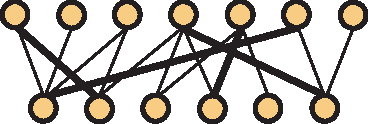
\includegraphics[scale=0.65,angle=90]{flowapplications-figs/bipartite_graph_part_match}
  \caption{A matching in a bipartite graph}
  \label{fig:flowapplications:bip_match}
\end{figure}


At the end of the chapter, we'll briefly look at a theorem on
matchings in bipartite graphs that tells us precisely when an
assignment of workers to jobs exists that ensures each worker has a
job. First, however, we want to see how network flows can be used to
find maximum matchings in bipartite graphs. The algorithm we give,
while decent, is not the most efficient algorithm known for this
problem. Therefore, it is not likely to be the one used in
practice. However, it is a nice example of how network flows can be
used to solve a combinatorial problem. The network that we use is
formed from a bipartite graph $\bfG$ by placing an edge from the
source $S$ to each vertex of $V_1$ and an edge from each vertex of
$V_2$ to the sink $T$. The edges between $V_1$ and $V_2$ are oriented
from $V_1$ to $V_2$, and \emph{every} edge is given capacity
$1$. \autoref{fig:flowapplications:bipmatch_network} contains the
network corresponding to our graph from
\autoref{fig:flowapplications:bip_graph}. Edges in this network are
all oriented from bottom to top and all edges have capacity $1$. The
vertices in $V_1$ are $x_1,\dots,x_6$ in order from left to right,
while the vertices in $V_2$ are $y_1,\dots, y_7$ from left to right.
\begin{figure}[ht]
  \centering
  \begin{overpic}[angle=90,scale=0.65]{flowapplications-figs/bipartite_network}
    \put(48,-6){$S$} \put(48,70){$T$}
    \put(9,13){$x_1$} %\put(38,74){$x_2$}
%    \put(38,60){$x_3$} \put(38,45){$x_4$}
%    \put(38,32){$x_5$} 
    \put(85,13){$x_6$}
    \put(3,56){$y_1$}% \put(61,81){$y_2$}
%    \put(61,67){$y_3$} \put(61,53){$y_4$}
%    \put(61,39){$y_5$} \put(61,25){$y_6$}
    \put(92,56){$y_7$}
  \end{overpic}
  \caption{The network corresponding to a bipartite graph}
  \label{fig:flowapplications:bipmatch_network}
\end{figure}

Now that we have translated a bipartite graph into a network, we need
to address the correspondence between matchings and network flows. To
turn a matching $M$ into a network flow, we start by placing one unit
of flow on the edges of the matching. To have a valid flow, we must
also place one unit of flow on the edges from $S$ to the vertices of
$V_1$ saturated by $M$. Since each of these vertices is incident with
a single edge of $M$, the flow out of each of them is $1$, matching
the flow in. Similarly, routing one unit of flow to $T$ from each of
the vertices of $V_2$ saturated by $M$ takes care of the conservation
laws for the remaining vertices. To go the other direction, simply
note that the full edges from $V_1$ to $V_2$ in an integer-valued flow
is a matching. Thus, we can find a maximum matching from $V_1$ to
$V_2$ by simply running the labeling algorithm on the associated
network in order to find a maximum flow.

In \autoref{fig:flowapplications:initial_flow}, we show thick edges to
show the edges with flow $1$ in the flow corresponding to our guess at
a matching from \autoref{fig:flowapplications:bip_match}.
\begin{figure}[ht]
  \centering
  \begin{overpic}[angle=90,scale=0.65]{flowapplications-figs/bipartite_network_flow}
    \put(48,-6){$S$} \put(48,70){$T$}
    \put(9,13){$x_1$} %\put(38,74){$x_2$}
%    \put(38,60){$x_3$} \put(38,45){$x_4$}
%    \put(38,32){$x_5$} 
    \put(85,13){$x_6$}
    \put(3,56){$y_1$}% \put(61,81){$y_2$}
%    \put(61,67){$y_3$} \put(61,53){$y_4$}
%    \put(61,39){$y_5$} \put(61,25){$y_6$}
    \put(92,56){$y_7$}
  \end{overpic}
  \caption{The flow corresponding to a matching}
  \label{fig:flowapplications:initial_flow}
\end{figure}
Now with priority sequence $S,T,x_1,x_2,\dots,x_6,y_1,y_2,\dots,y_7$
replacing our usual pseudo-alphabetic order, the labeling algorithm
produces the labels shown below.
\begin{align*}
  S:\quad &(*,+,\infty)&   y_6:\quad &(x_6,+,1)\\
  x_3:\quad &(S,+,1)&  x_1:\quad &(y_6,-,1)\\
  x_5:\quad &(S,+,1)&   y_1:\quad &(x_1,+,1)\\
  y_4:\quad &(x_3,+,1)&  y_2:\quad & (x_1,+,1)\\
  y_5:\quad &(x_3,+,1)&  y_3:\quad &(x_1,+,1)\\
  x_6:\quad &(y_4,-,1)&   x_2:\quad &(y_1,-,1)\\
  x_4:\quad &(y_5,-,1)&  T:\quad &(y_2,+,1)\\%
\end{align*}
This leads us to the augmenting path $S,x_3,y_4,x_6,y_6,x_1,y_2,T$,
which gives us the flow shown in \autoref{fig:flowapplications:bipmatch_maxflow}.
\begin{figure}[ht]
  \centering
  \begin{overpic}[angle=90,scale=0.65]{flowapplications-figs/bipartite_network_flow2}
    \put(48,-6){$S$} \put(48,70){$T$}
    \put(9,13){$x_1$} %\put(38,74){$x_2$}
%    \put(38,60){$x_3$} \put(38,45){$x_4$}
%    \put(38,32){$x_5$} 
    \put(85,13){$x_6$}
    \put(3,56){$y_1$}% \put(61,81){$y_2$}
%    \put(61,67){$y_3$} \put(61,53){$y_4$}
%    \put(61,39){$y_5$} \put(61,25){$y_6$}
    \put(92,56){$y_7$}
 \end{overpic}
  \caption{The augmented flow}
  \label{fig:flowapplications:bipmatch_maxflow}
\end{figure}
Is this a maximum flow? Another run of the labeling algorithm
produces
\begin{align*}
  S:\quad & (*,+,\infty)&  x_4:\quad & (y_5,-,1)\\
  x_5:\quad & (S,+,1)&  y_4:\quad &(x_4,+,1)\\
  y_5:\quad & (x_5,+,1)&  x_3:\quad &(y_4,-,1)
\end{align*}
and then halts. Thus, the flow in
\autoref{fig:flowapplications:bipmatch_maxflow} is a maximum flow.

Now that we know we have a maximum flow, we'd like to be able to argue
that the matching we've found is also maximum. After all, the boss
isn't going to be happy if he later finds out that this fancy
algorithm you claimed gave an optimal assignment of jobs to workers
left the fifth worker ($x_5$) without a job when all six of them could
have been put to work. Let's take a look at which vertices were
labeled by the Ford-Fulkerson labeling algorithm on the last
run. There were three vertices ($x_3$, $x_4$, and $x_5$) from $V_1$
labeled, while there were only two vertices ($y_4$ and $y_5$) from
$V_2$ labeled. Notice that $y_4$ and $y_5$ are the only vertices that
are neighbors of $x_3$, $x_4$, or $x_5$ in $\bfG$. Thus, no matter how
we choose the matching edges from $\{x_3,x_4,x_5\}$, one of these
vertices will be left unsaturated. Therefore, one of the workers must
go without a job assignment. (In our example, it's the fifth, but it's
possible to choose different edges for the matching so another one of
them is left without a task.)

The phenomenon we've just observed is not unique to our example. In
fact, in \emph{every} bipartite graph $\GVE$ with $V=V_1\cup V_2$ in
which we cannot find a matching that saturates all the vertices of $V$,
we will find a similar configuration. This is a famous theorem of
Hall, which we state below.

\begin{theorem}[Hall]\label{thm:flowapplications:hall}
  Let $\GVE$ be a bipartite graph with $V=V_1\cup V_2$. There is a
  matching which saturates all vertices of $V_1$ if and only if for
  every subset $A\subseteq V_1$, the set $N\subseteq V$ of neighbors
  of the vertices in $A$ satisfies $|N|\geq |A|$.
\end{theorem}
\section{Chain partitioning}

In \autoref{ch:posets}, we discussed
\hyperref[thm:dilworth]{Dilworth's theorem} (\autoref{thm:dilworth}),
which told us that for any poset $\bfP$ of width $w$, there is a
partition of $\bfP$ into $w$, but no fewer, chains. However, we were
only able to devise an algorithm to find this chain partition (and a
maximum antichain) in the special case where $\bfP$ was an interval
order. Now, through the magic of network flows, we will be able to
devise an efficient algorithm that works in general for all
posets. However, to do so, we will require a slightly more complicated
network than we devised in the previous section.

Suppose that the points of our poset $\bfP$ are
$\{x_1,x_2,\dots,x_n\}$. We construct a network from $\bfP$ consisting
of the source $S$, sink $T$, and two points $x'_i$ and $x''_i$ for
each point $x_i$ of $\bfP$. All edges in our network will have
capacity $1$. We add edges from $S$ to $x'_i$ for $1\leq i\leq n$ and
from $x''_i$ to $T$ for $1\leq i\leq n$. Of course, this network
wouldn't be too useful, as it has no edges from the single-prime nodes
to the double-prime nodes. To resolve this, we add an edge directed
from $x'_i$ to $x''_j$ if and only if $x_i < x_j$ in $\bfP$.

Our running example in this section will be the poset in
\hyperref[subfig:flowapplications:poset]{Figure \ref*{subfig:flowapplications:poset}}.  We'll discuss the points of the
poset as $x_i$ where $i$ is the number printed next to the point in
the diagram.
\begin{figure}[ht]\label{fig:flowapplications:poset}
  \centering
\begin{minipage}{1.3in}
      \subfloat[\label{subfig:flowapplications:poset}]{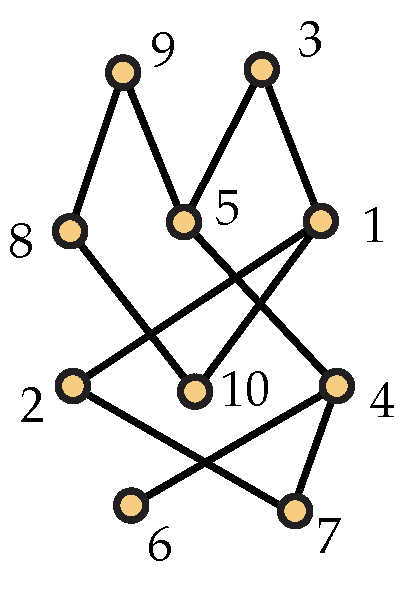
\includegraphics[width=1.1in]{flowapplications-figs/poset}}
  \end{minipage}\hspace{0.5in}
  \captionsetup[subfloat]{captionskip=15pt}
  \begin{minipage}{2.47in}
    \subfloat[\label{subfig:flowapplications:network}]{\begin{overpic}[angle=90,width=2.37in]{flowapplications-figs/poset_network}%
    \put(48,-5){$S$}%
    \put(48,93){$T$}%
    \put(1,20){$x_1'$}%
    \put(94,20){$x_{10}'$}%
    \put(1,71){$x_1''$}%
    \put(94,71){$x_{10}''$}%
 \end{overpic}}
  \end{minipage}
  \caption{A partially ordered set %
    \protect\subref{subfig:flowapplications:poset} and the associated network %
    \protect\subref{subfig:flowapplications:network}}
\end{figure}

The first step is to create the network, which we show in
\hyperref[subfig:flowapplications:network]{Figure~\ref*{subfig:flowapplications:network}}.
In this network, all capacities are $1$, edges are directed from
bottom to top, the first row of ten vertices is the $x'_i$ arranged
consecutively with $x'_1$ at the left and $x'_{10}$ at the right, and
the second row of ten vertices is the $x''_i$ in increasing order of
index. To see how this network is constructed, notice that $x_1<x_3$
in the poset, so we have the directed edge $(x_1',x_3'')$. Similarly,
$x_4$ is less than $x_3$, $x_5$, and $x_9$ in the poset, leading to
three directed edges leaving $x_4'$ in the network. As a third
example, since $x_9$ is maximal in the poset, there are no directed
edges leaving $x_9'$.

We have not yet seen how we might turn a maximum flow (or minimum cut)
in the network we've just constructed into a minimum chain partition
or a maximum antichain. It will be easier to see how this works once
we have a confirmed maximum flow. Rather than running the labeling
algorithm starting from the zero flow, we eyeball a flow, such as the
one shown in
\autoref{fig:flowapplications:poset_network_flow}. (Again, we use the
convention that thick edges are full, while thin edges are empty.)
\begin{figure}
  \centering
  \begin{overpic}[angle=90,scale=0.65]{flowapplications-figs/poset_network_flow}
    \put(48,-5){$S$}
    \put(48,93){$T$}
    \put(1,20){$x_1'$}
    \put(94,20){$x_{10}'$}
    \put(1,71){$x_1''$}
    \put(94,71){$x_{10}''$}

  \end{overpic}
   \caption{ An initial flow}
    \label{fig:flowapplications:poset_network_flow}
\end{figure}
When we run the labeling algorithm (using priority
$S,T,x_1',\dots,x_{10}',x_1'',\dots,x_{10}''$), we obtain the
following list of labels:
 \begin{align*}
  S:\quad &(*,+,\infty) & x''_9:\quad &(x'_5,+,1) & x'_3:\quad &(S,+,1)   \\
  x'_3:\quad &(S,+,1) & x''_4:\quad &(x'_6,+,1) &x''_1:\quad &(x'_7,+,1)    \\
  x'_5:\quad &(S,+,1)& x''_5:\quad &(x'_6,+,1) & x''_2:\quad &(x'_7,+,1)  \\
  x'_6:\quad &(S,+,1)& x'_1:\quad &(x''_3,-,1) & x'_2:\quad &(x'_7,+,1)  \\
  x'_9:\quad &(S,+,1)& x'_8:\quad &(x''_9,-,1) & T:\quad &(x''_2,+,1)  \\
  x''_3:\quad &(x'_5,+,1) & x'_7:\quad &(x''_4,-,1)  & \\
\end{align*}
Thus, we find the augmenting path $(S,x'_6,x''_4,x'_7,x''_2,T)$, and the
updated flow can be seen in \autoref{fig:flowapplications:poset_network_flow2}.
\begin{figure}[ht]
  \centering
  \begin{overpic}[angle=90,scale=0.65]{flowapplications-figs/poset_network_flow2}
    \put(48,-5){$S$}
    \put(48,93){$T$}
    \put(1,20){$x_1'$}
    \put(94,20){$x_{10}'$}
    \put(1,71){$x_1''$}
    \put(94,71){$x_{10}''$}

  \end{overpic}
 \caption{ A better flow}
  \label{fig:flowapplications:poset_network_flow2}
\end{figure}
If we run the labeling algorithm again, the algorithm assigns the labels
below, leaving the sink unlabeled.
\begin{align*}
  S:\quad & (*,+,\infty)& x'_5:\quad &(S,+,1) & x''_3:\quad
  &(x'_5,+,1) & x'_1:\quad & (x''_3,-,1)\\
  x'_3:\quad &(S,+,1) & x'_9:\quad &(S,+,1) & x''_9:\quad & (x'_5,+,1)
  & x'_8:\quad &(x''_9,-,1)
\end{align*}
In \autoref{fig:flowapplications:poset_network_flow2}, the black
vertices are those the labeled in the final run, while the gold
vertices are the unlabeled vertices.

Now that we've gone over the part you already knew how to do, we need
to discuss how to translate this network flow and cut into a chain
partition and an antichain. If there is a unit of flow on an edge
$(x_i',x_j'')$, then a good first instinct is to place $x_i$ and $x_j$
in the same chain of a chain partition. To be able to do this
successfully, of course, we need to ensure that this won't result in
two incomparable points being placed in a chain. A way to see that
everything works as desired is to think of starting with
$(x_i',x_j'')$ and then looking for flow leaving $x_j'$. If there is,
it goes to a vertex $x_k''$, so we may add $x_k$ to the chain since
$x_i<x_j<x_k$. Continue in this manner until reaching a vertex in the
network that does not have any flow leaving it. Then see if $x_i''$
has flow coming into it. If it does, it's from a vertex $x_m'$ that
can be added since $x_m<x_i<x_j$.

Let's see how following this process for the flow in
\autoref{fig:flowapplications:poset_network_flow2} leads to a chain
partition. If we start with $x_1'$, we see that $(x_1',x_3'')$ is
full, so we place $x_1$ and $x_3$ in chain $C_1$. Since $x_3'$ has no
flow leaving it, there are no greater elements to add to the
chain. However, $x_1''$ has flow in from $x_2'$, so we add $x_2$ to
$C_1$. We now see that $x_2''$ has flow in from $x_7'$, so now
$C_1=\{x_1,x_2,x_3,x_7\}$. Vertex $x_7''$ has no flow into it, so the
building of the first chain stops. The first vertex we haven't placed
into a chain is $x_4$, so we note that $(x_4',x_5'')$ is full, placing
$x_4$ and $x_5$ in chain $C_2$. We then look from $x_5'$ and see no
flow leaving. However, there is flow into $x_4''$ from $x_6'$, so
$x_6$ is added to $C_2$. There is no flow out of $x_6''$, so
$C_2=\{x_4,x_5,x_6\}$. Now the first point not in a chain is $x_8$, so
we use the flow from $x_8'$ to $x_9''$ to place $x_8$ and $x_9$ in
chain $C_3$. Again, no flow out of $x_9'$, so we look to $x_8''$,
which is receiving flow from $x_{10}''$. Adding $x_{10}$ to $C_3$
gives $C_3=\{x_8,x_9,x_{10}\}$, and since every point is now in a
chain, we may stop.

Even once we see that the above process does in fact generate a chain
partition, it is not immediately clear that it's a minimum chain
partition. For this, we need to find an antichain of as many points as
there are chains in our partition. (In the example we've been using,
we need to find a three-element antichain.) This is where tracking
the labeled vertices comes in handy. Suppose we have determined a
chain $C=\{x_1<x_2<\cdots < x_k\}$ using the network flow. Since $x_1$
is the minimal element of this chain, there is no flow into $x_1''$
and hence no flow out of $x_1''$. Since $T$ is unlabeled, this must
mean that $x_1''$ is unlabeled. Similarly, $x_k$ is the maximal
element of $C$, so there is no flow out of $x_k'$. Thus, $x_k'$ is
labeled. Now considering the sequence of vertices
\[x_k',x_k'',x_{k-1}',x_{k-1}'',\dots,x_2',x_2'',x_1',x_1'',\] there
must be a place where the vertices switch from being labeled to
unlabeled. This must happen with $x_i'$ labeled and $x_i''$
unlabeled. To see why, suppose that $x_i'$ and $x_i''$ are both
unlabeled while $x_{i+1}'$ and $x_{i+1}''$ are both labeled. Because
$x_i$ and $x_{i+1}$ are consecutive in $C$, there is flow on
$(x_i',x_{i+1}'')$. Therefore, when scanning from $x_{i+1}''$, the
vertex $x_i'$ would be labeled. For each chain of the chain partition,
we then take the first element $y$ for which $y'$ is labeled and $y''$
is unlabeled to form an antichain $A=\{y_1,\dots,y_w\}$. To see that
$A$ is an antichain, notice that if $y_i<y_j$, then $(y_i',y_j'')$ is
an edge in the network. Therefore, the scan from $y_i'$ would label
$y_j''$. Using this process, we find that a maximum antichain in our
example is $\{x_1,x_5,x_8\}$.

\section{Exercises}

\begin{enumerate}
\item Use the techniques of this chapter to find a maximum matching
  from $V_1$ to $V_2$ in the graph shown in
  \autoref{fig:flowapplications:matching_ex1}. The vertices on the
  bottom are the set $V_1$, while the vertices on the top are the set
  $V_2$. If you cannot find a matching that saturates all of the
  vertices in $V_1$, explain why.
  \begin{figure}[h]
    \centering
    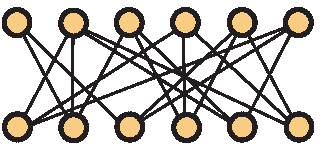
\includegraphics[scale=0.6]{flowapplications-figs/matching_ex1}
    \caption{Is there a matching saturating $V_1$?}
    \label{fig:flowapplications:matching_ex1}
  \end{figure}
\item Use the techniques of this chapter to find a maximum matching
  from $V_1$ to $V_2$ in the graph shown in
  \autoref{fig:flowapplications:matching_ex2}. The vertices on the
  bottom are the set $V_1$, while the vertices on the top are the set
  $V_2$. If you cannot find a matching that saturates all of the
  vertices in $V_1$, explain why.
  \begin{figure}[h]
    \centering
    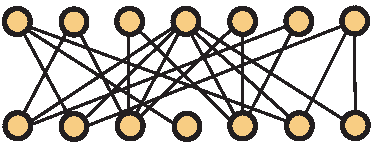
\includegraphics[scale=0.6]{flowapplications-figs/matching_ex2}
    \caption{Is there a matching saturating $V_1$?}
    \label{fig:flowapplications:matching_ex2}
  \end{figure}
\item Students are preparing to do final projects for an applied
  combinatorics course. The five possible topics for their final
  projects are graph algorithms, posets, induction, graph theory, and
  generating functions. There are five students in the class, and they
  have each given their professor the list of topics on which they are
  willing to do their project. Alice is interested in posets or
  graphs. Bob would be willing to do his project on graph algorithms,
  posets, or induction. Carlos will only consider posets or
  graphs. Dave likes generating functions and induction. Yolanda wants to
  do her project on either graphs or posets.  To prevent unauthorized
  collaboration, the professor does not want to have two students work
  on the same topic. Is it possible to assign each student a topic
  from the lists above so that no two students work on the same
  project? If so, find such an assignment. If not, find an assignment
  that maximizes the number of students who have assignments from
  their lists and explain why you cannot satisfy all the students'
  requests.
\item Seven colleges and universities are competing to recruit six
  high school football players to play for their varsity teams. Each
  school is only allowed to sign one more player, and each player is
  only allowed to commit to a single school. The table below lists the
  seven institutions and the students they are trying to recruit, have
  been admitted, and are also interested in playing for that
  school. (There's no point in assigning a school a player who cannot
  meet academic requirements or doesn't want to be part of that team.)
  The players are identified by the integers $1$ through $6$.  Find a
  way of assigning the players to the schools that maximizes the
  number of schools who sign one of the six players.
  \begin{center}
    \begin{tabular}{r|l}
      School & Player numbers\\\hline
      Boston College & 1, 3, 4\\
      Clemson University & 1, 3, 4, 6\\
      Georgia Institute of Technology & 2, 6\\
      University of Georgia & None interested\\
      University of Maryland & 2, 3, 5\\
      University of North Carolina & 1, 2, 5\\
      Virginia Polytechnic Institute and State University & 1, 2, 5, 6
    \end{tabular}
  \end{center}
\item The questions in this exercise refer to the network diagram in
  \autoref{fig:flowapplications:poset_network_ex1}. This network
  corresponds to a poset $\bfP$. As usual, all
  capacities are assumed to be $1$, and all edges are directed
  upward. Answer the following questions about $\bfP$ \emph{without
    drawing the diagram of the poset}.
  \begin{enumerate}
  \item Which element(s) are greater than $x_1$ in $\bfP$?
  \item Which element(s) are less than $x_5$ in $\bfP$?
  \item Which element(s) are comparable with $x_6$ in $\bfP$?
  \item List the maximal elements of $\bfP$.
  \item List the minimal elements of $\bfP$.
  \end{enumerate}
 \begin{figure}[h]
    \centering
    \begin{overpic}[scale=0.6]{flowapplications-figs/poset_network_ex1}
      \put(47,-7){$S$}
      \put(47,91){$T$}
      \put(3,15){$x_1'$}      \put(90,15){$x_6'$}
      \put(3,70){$x_1''$}      \put(90,70){$x_6''$}
    \end{overpic}
    \caption{The network corresponding to a poset}
    \label{fig:flowapplications:poset_network_ex1}
  \end{figure}
\item Draw the diagram of the poset that corresponds to the network in
  \autoref{fig:flowapplications:poset_network_ex1}.
\item Use the methods developed in this chapter to find the width $w$
  of the poset corresponding to the network in
  \autoref{fig:flowapplications:poset_network_ex1}. Also find an
  antichain of size $w$ and a partition into $w$ chains.
\item In \autoref{fig:flowapplications:poset_network_ex} we show a
  poset $\bfP$ and a network used to find a chain partition of
  $\bfP$. (All edges in the network have a capacity of $1$ and are
  directed from bottom to top. The \textbf{bold} edges currently carry
  a flow of $1$.) Using the network, find the width $w$ of $\bfP$, a
  partition of $\bfP$ into $w$ chains, and an antichain with $w$
  elements.
  \begin{figure}[h]
    \centering
    \begin{overpic}[scale=0.5]{flowapplications-figs/chain-partition}
      \put(2,21){$x_1$}
      \put(32,25){$x_2$}
      \put(17,21){$x_3$}
      \put(19,38){$x_4$}
      \put(1,1){$x_5$}
      \put(23,0){$x_6$}
      \put(69.5,-2){$S$}
      \put(69.5,42){$T$}
      \put(48,7){$x'_1$}
      \put(91,7){$x'_6$}
      \put(48,33){$x''_1$}
      \put(91,33){$x''_6$}
    \end{overpic}
    \caption{A poset and the corresponding network diagram}
    \label{fig:flowapplications:poset_network_ex}
  \end{figure}
  \begin{center}

  \end{center}
\item Draw the network corresponding to the poset $\bfP$ shown in
  \autoref{fig:flowapplications:poset_ex}. Use the network to find the
  width $w$ of $\bfP$, a partition into $w$ chains, and an antichain
  of size $w$.
  \begin{figure}[h]
    \centering
    \begin{overpic}[scale=0.5]{flowapplications-figs/poset_ex}
      \put(55,48){$x_1$}
      \put(45,-2){$x_2$}
      \put(27,72){$x_3$}
      \put(59,80){$x_4$}
      \put(28,33){$x_5$}
      \put(79,54){$x_6$}
      \put(87,3){$x_7$}
      \put(0,54){$x_8$}
      \put(57,27){$x_9$}
      \put(94,31){$x_{10}$}
    \end{overpic}
    \caption{A poset}
    \label{fig:flowapplications:poset_ex}
  \end{figure}

\end{enumerate}

%%% Local Variables: 
%%% mode: latex
%%% TeX-master: "book"
%%% End: 
